\chapter{Simulation}
Output measurement with harmonic balance simulator in agilent design system in time domain for a frequency of 1 GHz.
Simulation  with ADS. \\Harmonic Balance simulation for the steady-state.\\ S-param for the matching.\\ Stability that no oscillation occurs. \\ energy consumption\\

Three different signals should be synthesized using the digital-to-analog converter named Riemann Pump. This signals were generated with a resolution of 3-bit. 
\begin{enumerate}
	\item sine wave
	\item half sine wave
	\item triangular wave
\end{enumerate}
All signals are generated using a oversampling ratio of four, $OSR = 2^{r} = 4$. Hence the factor $r = 2$ which is used in the diagrams provided by the french mathematics. The digital control sequence is based on the weights of the slopes and the riemann code is generated by hand. Therefore no matlab script exists which calculates the optimal code, minimizing the error, for controlling the digital to analog converter. 

%% Important: appearance all the same, same frequency, sam oversamplingratio, same resolution, et cetera
% create this figure/picture
\begin{figure}[ht]
	\centering
  \includegraphics[width=1\textwidth, draft]{DAC_generated_sine_wave.png}
	\caption{Digital to analog converted signal representing a sine wave using ads simulation}
	\label{DAC_generated_sine_wave}
\end{figure}

\begin{figure}[ht]
	\centering
  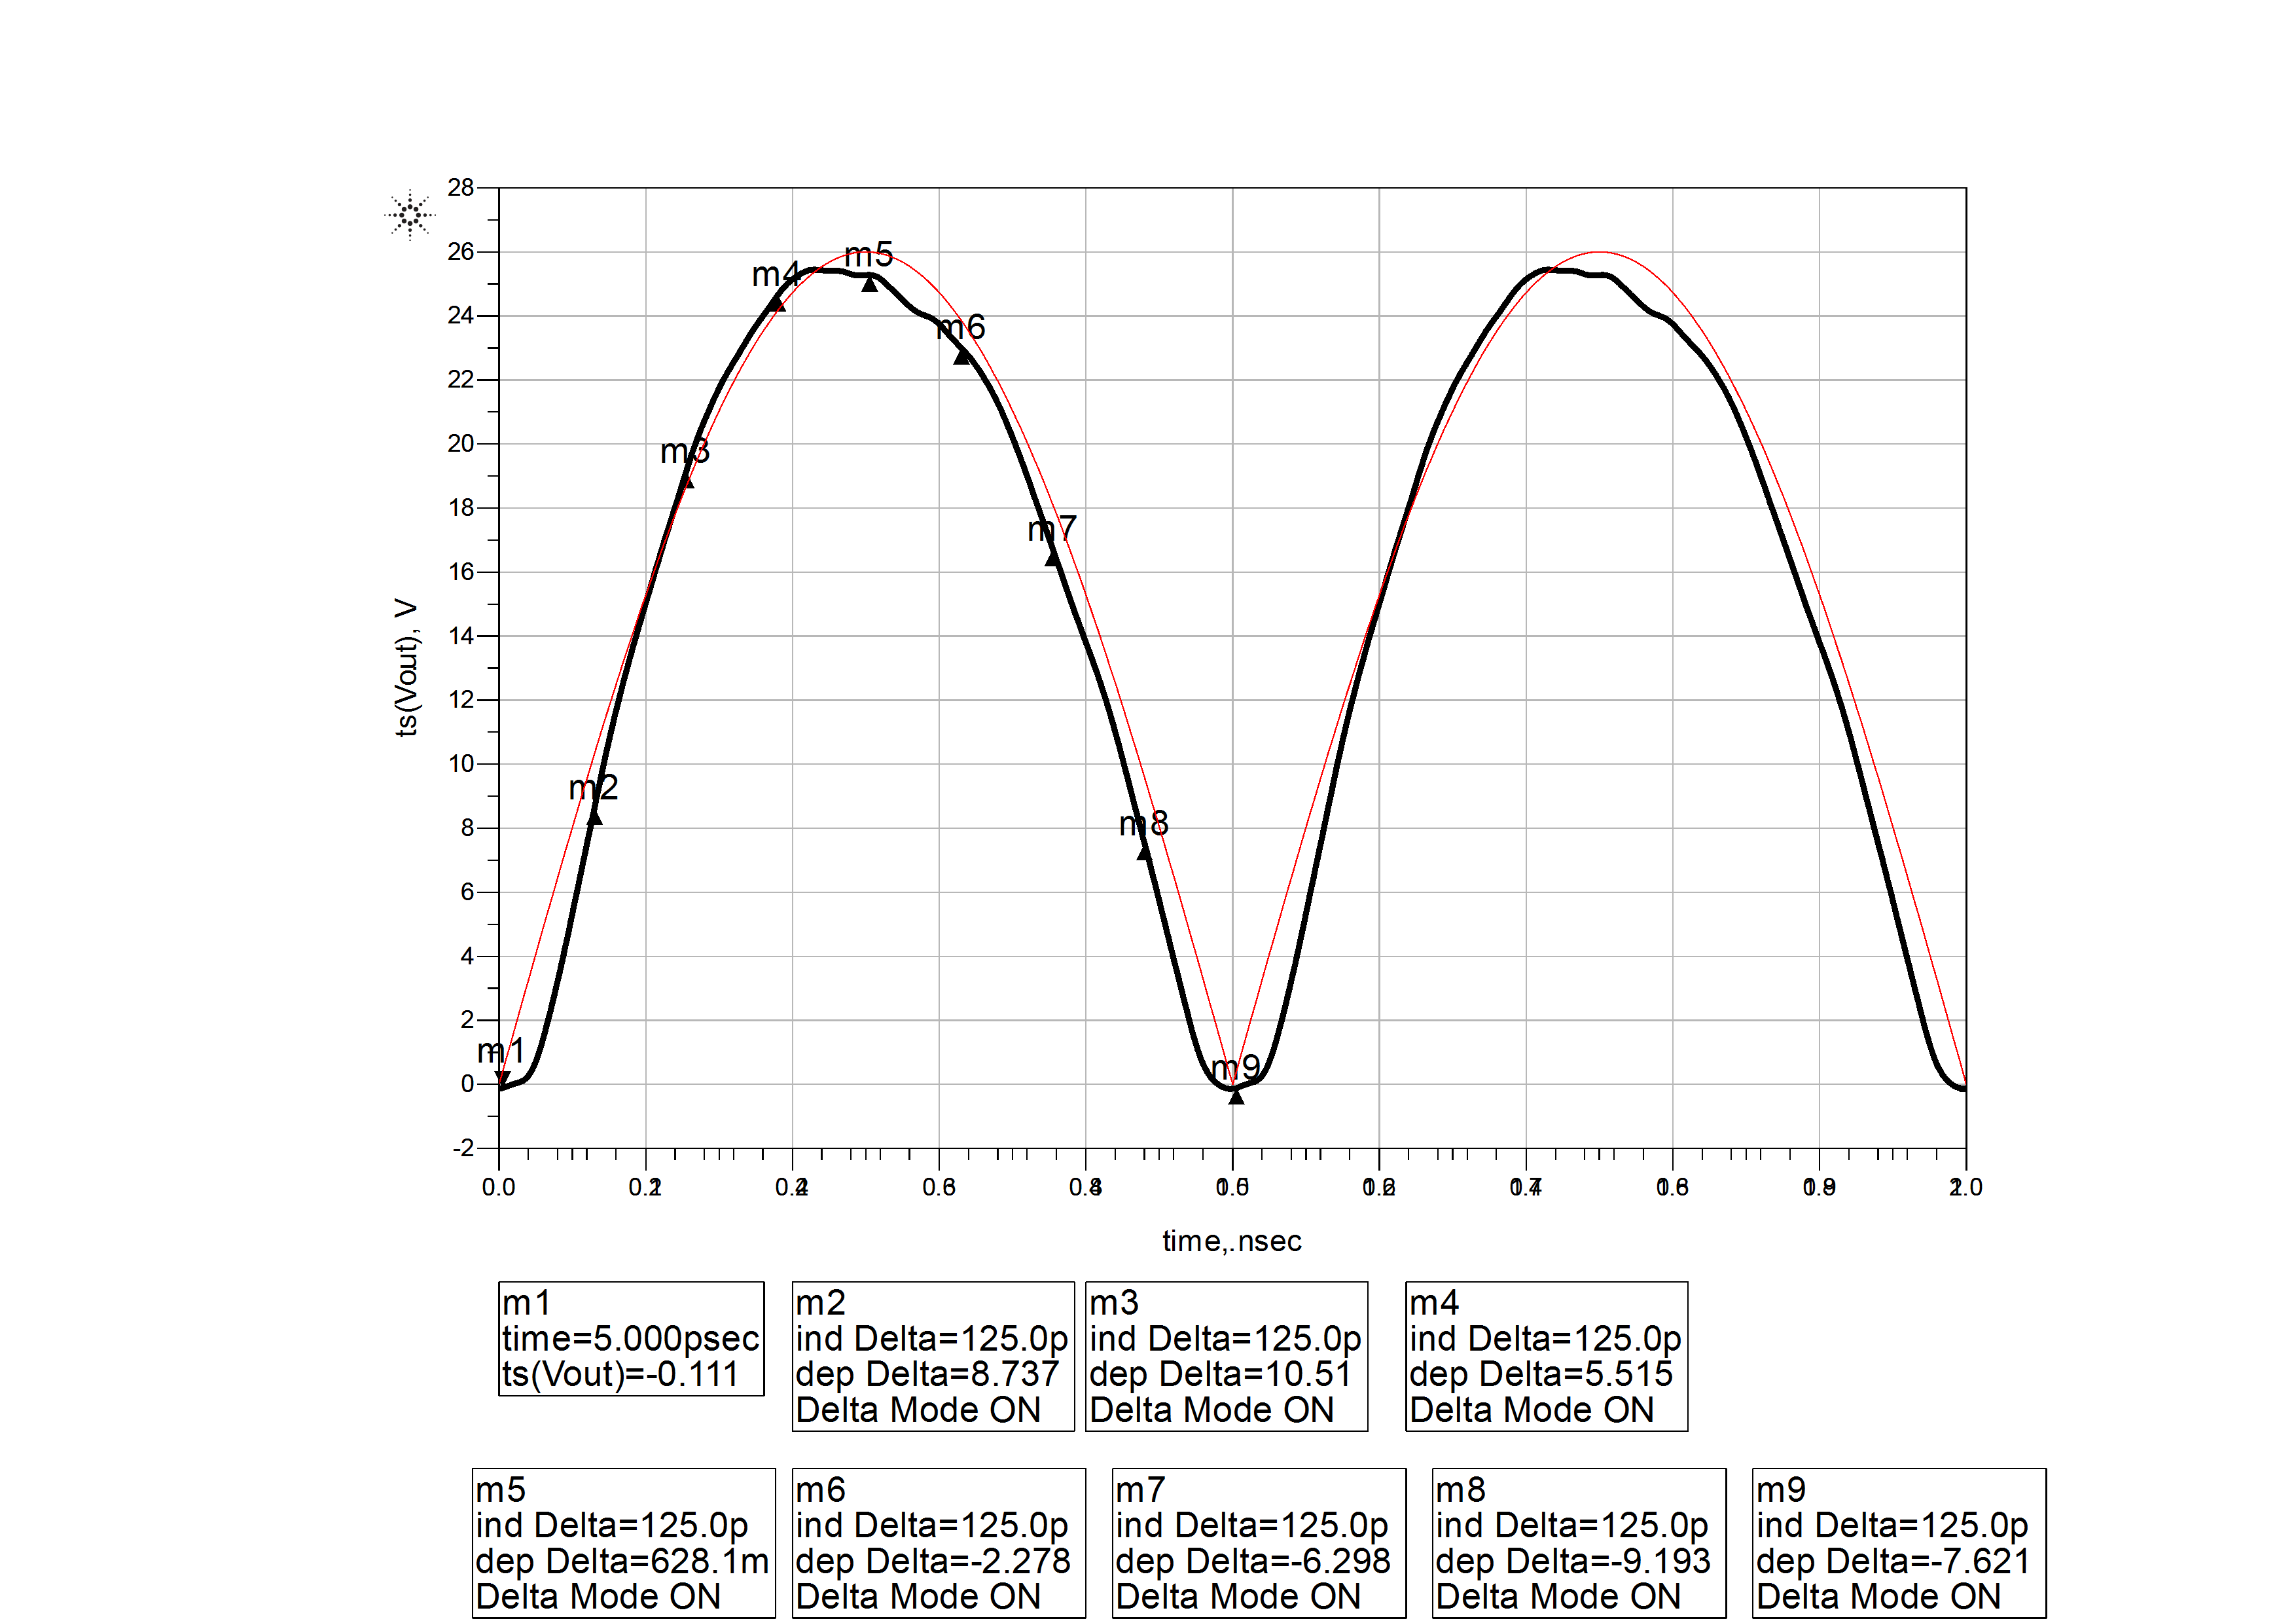
\includegraphics[width=1\textwidth, draft]{halfsine_generated_1GHz.png}
	\caption{Digital to analog converted signal representing a sine half wave and a theoretical signal to compare the signal to noise ratio}
	\label{halfsine}
\end{figure}

\begin{figure}[ht]
	\centering
  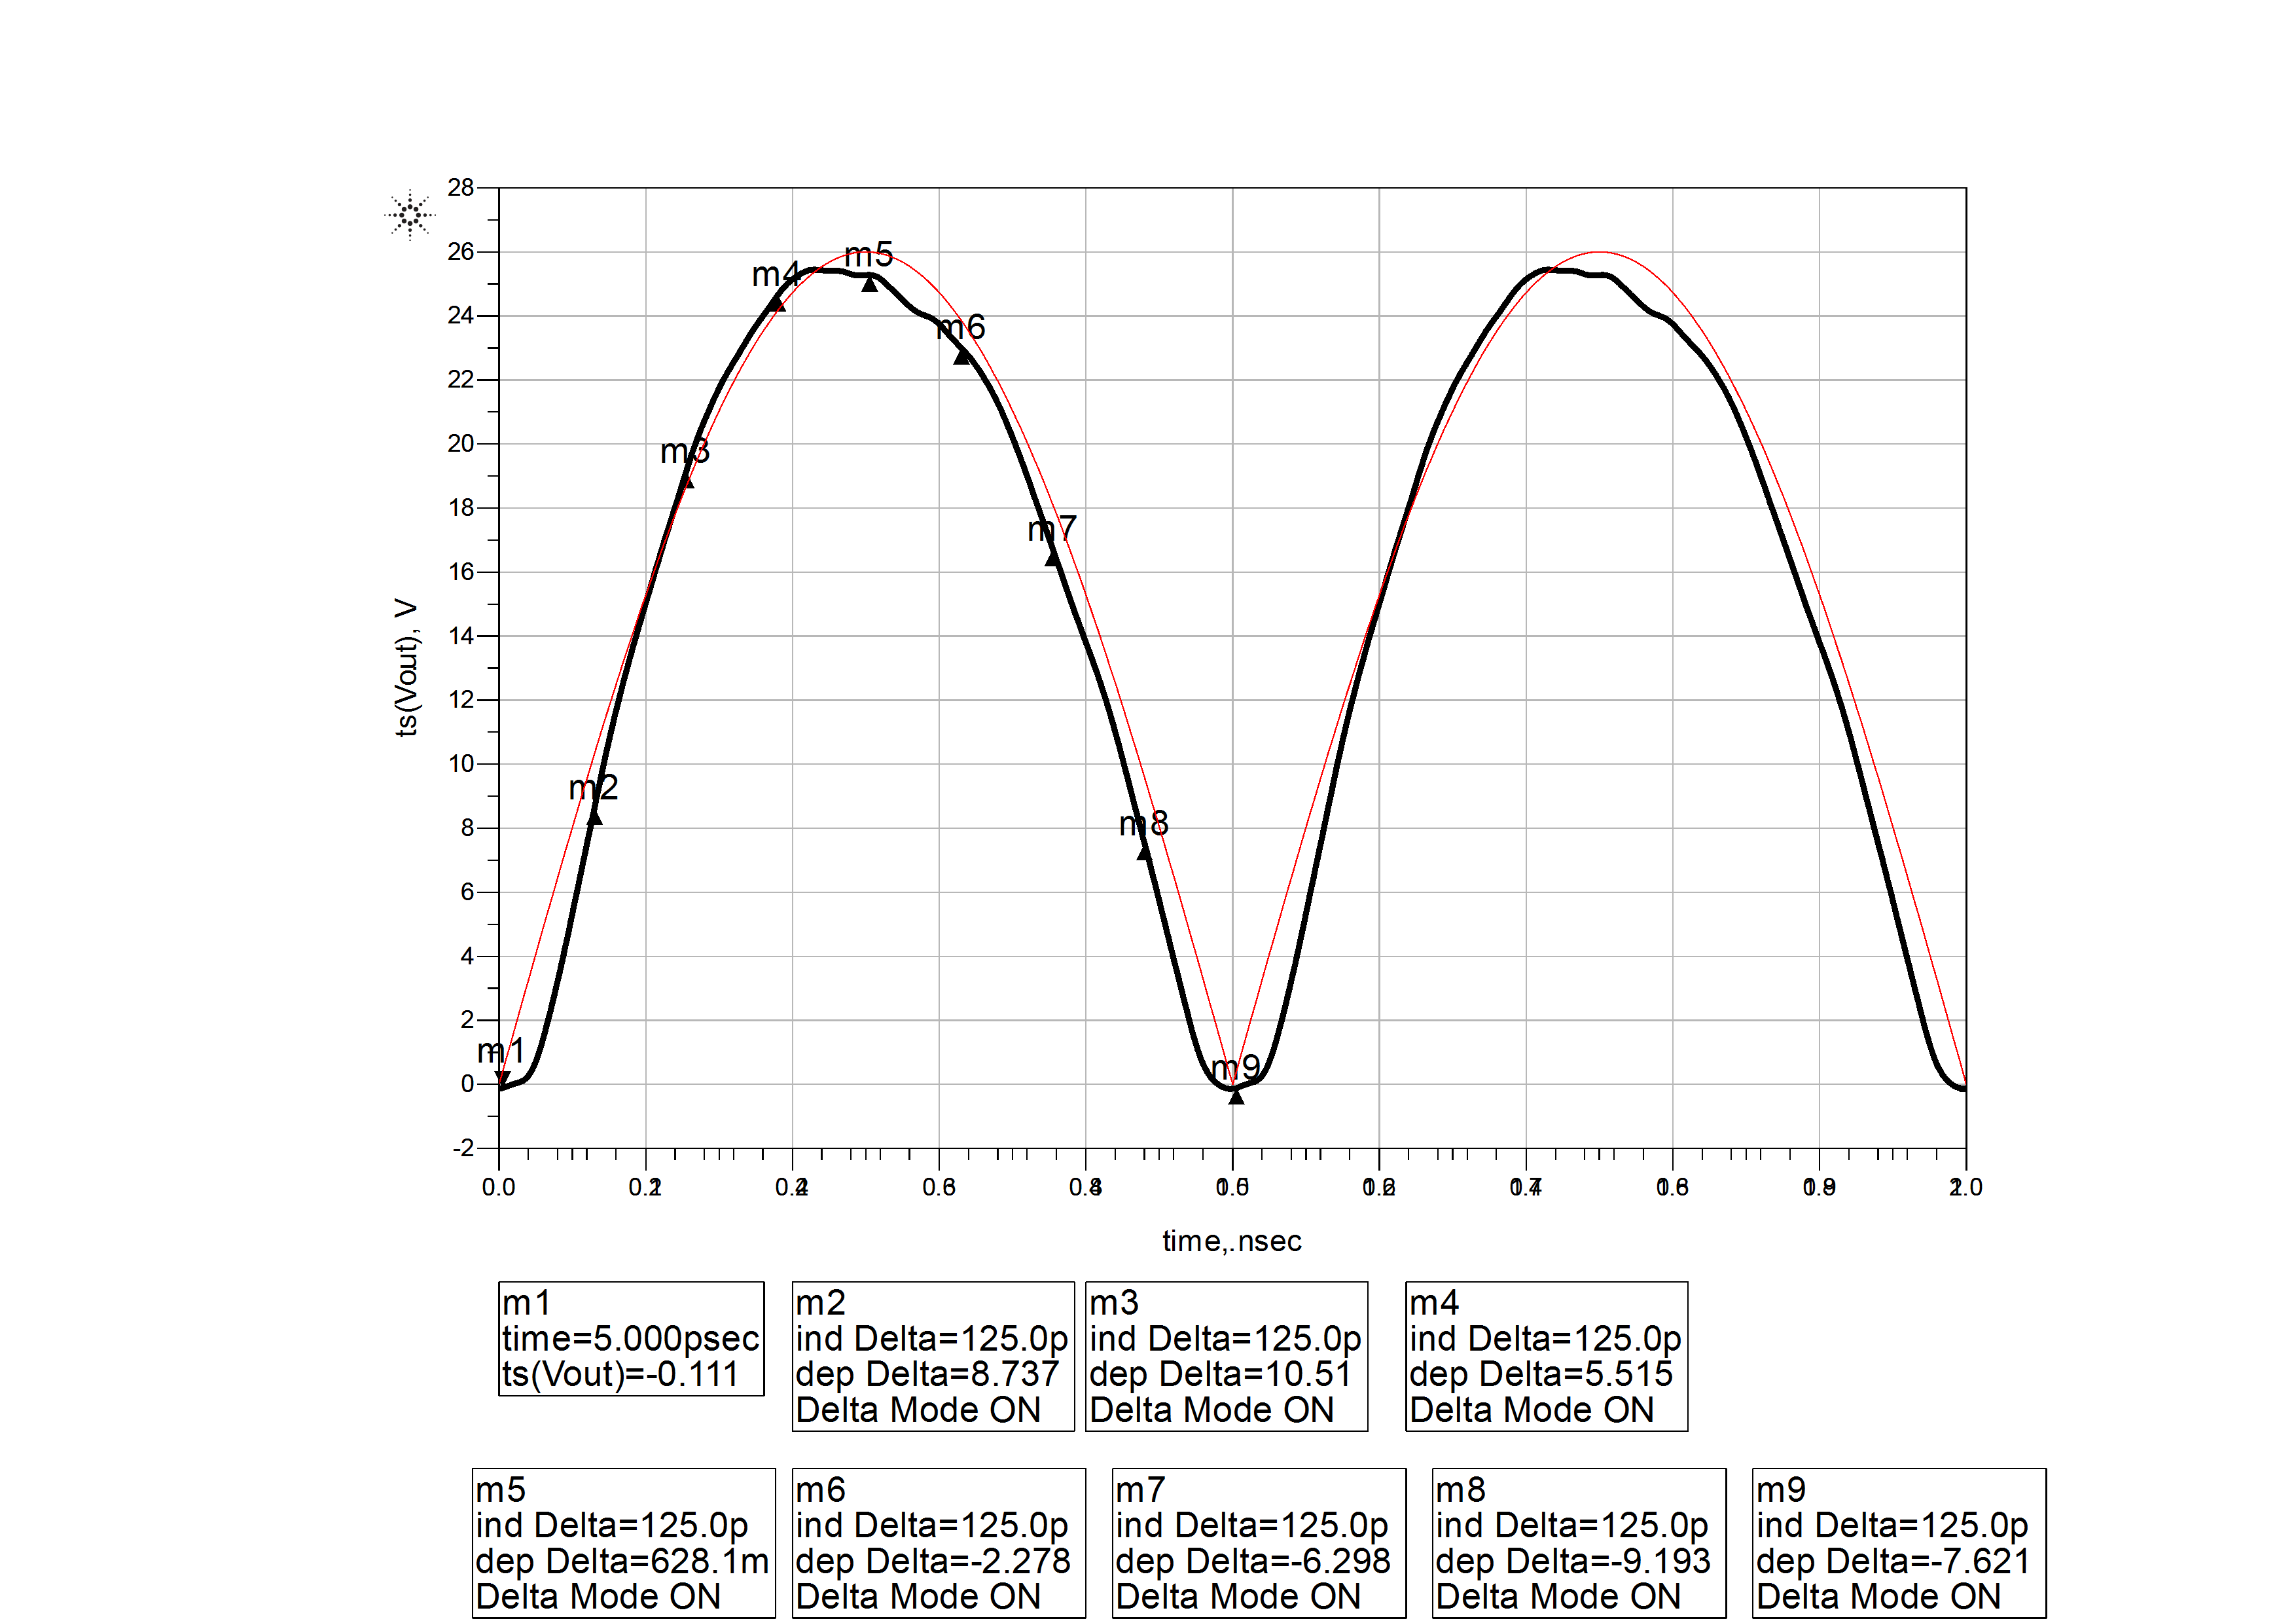
\includegraphics[width=1\textwidth, draft]{halfsine_generated_1GHz.png}
	\caption{Digital to analog converted signal representing a sine half wave and a theoretical signal to compare the signal to noise ratio}
	\label{halfsine}
\end{figure}